\documentclass[11pt,a4paper]{article}

% ---------- packages ----------
\usepackage{amsmath,amsthm}
\usepackage{libertine}
\usepackage[libertine]{newtxmath}
\usepackage[a4paper,margin=2.4cm]{geometry}
\usepackage{booktabs,array}
\usepackage{cancel}
\usepackage{xcolor}
\usepackage{tikz}
\usetikzlibrary{arrows.meta,calc,positioning}
\usepackage{tcolorbox}
\usepackage{enumitem}
\usepackage{microtype}
\usepackage[colorlinks=true,linkcolor=blue!50!black,urlcolor=blue!50!black,citecolor=blue!50!black]{hyperref}

% ---------- notation ----------
\newcommand{\ket}[1]{\lvert #1 \rangle}
\newcommand{\bra}[1]{\langle #1 \rvert}
\newcommand{\RX}{R_X}
\newcommand{\RY}{R_Y}
\newcommand{\CRX}{CR_X}
\newcommand{\Z}{\mathbb{Z}}
\newcommand{\C}{\mathbb{C}}
\newcommand{\code}[1]{\texttt{#1}}
\newcommand{\eqmod}[1]{\;\equiv\;#1\pmod{2\pi}}

\theoremstyle{plain}
\newtheorem{lemma}{Lemma}[section]
\newtheorem{theorem}[lemma]{Theorem}
\theoremstyle{definition}
\newtheorem{definition}[lemma]{Definition}
\theoremstyle{remark}
\newtheorem{remark}[lemma]{Remark}

\definecolor{gatecol}{HTML}{9F1853}
\definecolor{keycol}{HTML}{0F62FE}
\newtcolorbox{keybox}[1][Key idea]{colback=keycol!4,colframe=keycol!70!black,fonttitle=\bfseries,title=#1,sharp corners,boxrule=0.6pt,left=6pt,right=6pt,top=4pt,bottom=4pt}
\newtcolorbox{resultbox}[1][Architecture result]{colback=gatecol!4,colframe=gatecol,fonttitle=\bfseries,title=#1,sharp corners,boxrule=0.6pt,left=6pt,right=6pt,top=4pt,bottom=4pt}

\tikzset{
  wire/.style={thick},
  gate/.style={draw=gatecol,fill=gatecol!12,thick,minimum width=1.55cm,minimum height=0.8cm,font=\small,inner sep=2pt},
  ctrl/.style={circle,fill=gatecol,inner sep=0pt,minimum size=6pt},
  meas/.style={draw,thick,minimum width=0.8cm,minimum height=0.8cm,fill=white},
}

\title{\textbf{The Super Parameter}\\[4pt]
\large Deriving a One-Parameter Quantum Circuit from Binary Arithmetic}
\author{Oussema-t\\[2pt]\small\href{https://github.com/Oussema-t/pennylane-super-parameter}{github.com/Oussema-t/pennylane-super-parameter}}
\date{September 2026}

\begin{document}
\maketitle

\begin{abstract}
\noindent
The PennyLane challenge \emph{The Super Parameter} asks for a three-qubit circuit with a
\emph{single} parameter $\alpha$ that can produce every one of the eight computational basis
states $\ket{000},\dots,\ket{111}$. This document derives such a circuit from scratch. The only
tools needed are the binary expansion $n = 4b_0 + 2b_1 + b_2$, the fact that an $\RX$ rotation
lands on a basis state exactly when its angle is a whole multiple of $\pi$, and the observation
that a rotation by $2\pi$ changes nothing observable. Three lines of modular arithmetic then
force every gate, every angle and every control wire of the circuit. We prove each step, verify
the result for all eight inputs, walk through one input state by state, and prove that no circuit
made of uncontrolled rotations alone could do the job. No prior knowledge of quantum computing
is assumed beyond comfort with vectors, complex numbers and trigonometry.
\end{abstract}

{\setcounter{tocdepth}{1}\tableofcontents}
\clearpage

% =====================================================================
\section{The problem in plain words}
% =====================================================================

A qubit is the quantum version of a bit. Three qubits together have eight ``classical''
configurations, written as three-digit binary strings:
\[
\ket{000},\ \ket{001},\ \ket{010},\ \ket{011},\ \ket{100},\ \ket{101},\ \ket{110},\ \ket{111}.
\]
Reading each string as a binary number gives the integers $0,1,\dots,7$. These eight
configurations are called the \emph{computational basis states}.

The challenge is the following. Build a quantum circuit on three qubits whose gates depend on
one real number $\alpha$ (the ``super parameter''). Then provide eight values
$\alpha_0,\dots,\alpha_7$, all in the interval $[0,10]$, such that running the circuit with
$\alpha_n$ produces exactly the basis state with binary value $n$. The circuit must also be
\emph{continuous} in $\alpha$: a small change of the knob must produce a small change of the
output. Putting $\alpha$ inside rotation angles guarantees this automatically.

With three independent knobs the task would be trivial: one rotation per qubit, each turned to
$0$ or $\pi$. With one knob it is not obvious at all, because the same number must simultaneously
steer three qubits to three different, independent targets. The solution is the circuit in
Figure~\ref{fig:circuit}, and the values are simply $\alpha_n = n$.

\begin{figure}[ht]
\centering
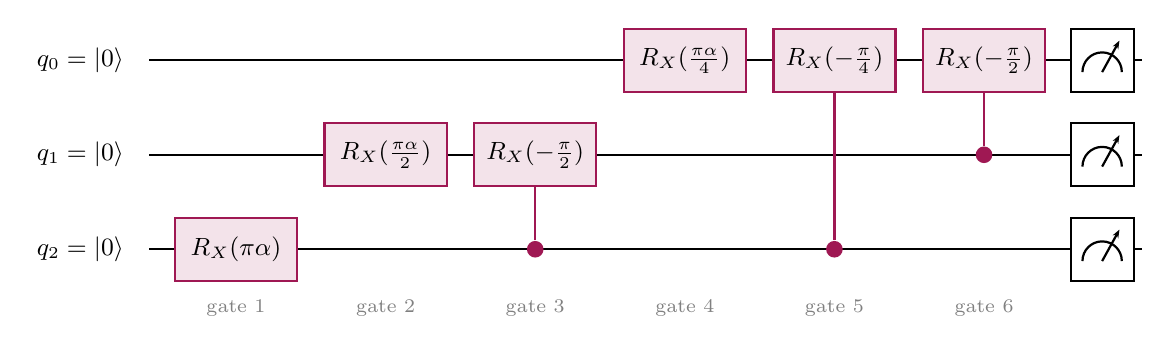
\begin{tikzpicture}[x=1cm,y=1cm]
  % wires
  \foreach \k/\y in {0/2.4,1/1.2,2/0} {
    \node[anchor=east,font=\small] at (-0.2,\y) {$q_{\k}=\ket{0}$};
    \draw[wire] (0,\y) -- (12.6,\y);
  }
  % gate 1: RX(pi a) on q2
  \node[gate] (g1) at (1.1,0) {$\RX(\pi\alpha)$};
  % gate 2: RX(pi a/2) on q1
  \node[gate] (g2) at (3.0,1.2) {$\RX(\tfrac{\pi\alpha}{2})$};
  % gate 3: CRX(-pi/2) 2->1
  \node[gate] (g3) at (4.9,1.2) {$\RX(-\tfrac{\pi}{2})$};
  \node[ctrl] (c3) at (4.9,0) {};
  \draw[thick,gatecol] (c3) -- (g3.south);
  % gate 4: RX(pi a/4) on q0
  \node[gate] (g4) at (6.8,2.4) {$\RX(\tfrac{\pi\alpha}{4})$};
  % gate 5: CRX(-pi/4) 2->0
  \node[gate] (g5) at (8.7,2.4) {$\RX(-\tfrac{\pi}{4})$};
  \node[ctrl] (c5) at (8.7,0) {};
  \draw[thick,gatecol] (c5) -- (g5.south);
  % gate 6: CRX(-pi/2) 1->0
  \node[gate] (g6) at (10.6,2.4) {$\RX(-\tfrac{\pi}{2})$};
  \node[ctrl] (c6) at (10.6,1.2) {};
  \draw[thick,gatecol] (c6) -- (g6.south);
  % measurement
  \foreach \y in {2.4,1.2,0} {
    \node[meas] (m) at (12.1,\y) {};
    \draw[thick] ($(m.center)+(-0.25,-0.15)$) arc[start angle=180,end angle=0,radius=0.25];
    \draw[thick,-{Stealth[length=3pt]}] ($(m.center)+(0,-0.15)$) -- ($(m.center)+(0.22,0.25)$);
  }
  % step numbers
  \foreach \x/\n in {1.1/1,3.0/2,4.9/3,6.8/4,8.7/5,10.6/6} {
    \node[font=\scriptsize,gray] at (\x,-0.75) {gate \n};
  }
\end{tikzpicture}
\caption{The solution circuit. Filled dots are control qubits: the attached rotation is applied
to the target wire only when the control qubit is $\ket{1}$. Wire $q_0$ is the most-significant
bit of the output, $q_2$ the least-significant bit. The gates are numbered in the order they are
applied.}
\label{fig:circuit}
\end{figure}

In PennyLane the circuit reads:
\begin{quote}\small
\begin{verbatim}
@qml.qnode(dev)
def model(alpha):
    qml.RX(np.pi * alpha, wires=2)
    qml.RX(np.pi * alpha / 2, wires=1)
    qml.CRX(-np.pi / 2, wires=[2, 1])
    qml.RX(np.pi * alpha / 4, wires=0)
    qml.CRX(-np.pi / 4, wires=[2, 0])
    qml.CRX(-np.pi / 2, wires=[1, 0])
    return qml.probs(wires=[0, 1, 2])

def generate_coefficients():
    return [0, 1, 2, 3, 4, 5, 6, 7]
\end{verbatim}
\end{quote}

The rest of this document explains where every piece of this circuit comes from.
Section~\ref{sec:qm} collects the small amount of quantum mechanics we need.
Section~\ref{sec:arith} turns the problem into a statement about angles.
Section~\ref{sec:derivation} is the heart: the derivation of the three wires.
Section~\ref{sec:check} verifies all eight cases, Section~\ref{sec:example} follows one input
through the circuit state by state, Section~\ref{sec:rigor} makes the ``cross out $2\pi$'' step
rigorous, and Section~\ref{sec:impossible} proves that controlled gates cannot be avoided.

% =====================================================================
\section{Just enough quantum mechanics}\label{sec:qm}
% =====================================================================

\subsection{One qubit}

A qubit's state is a vector in $\C^2$ of length one. The two basis vectors are written
\[
\ket{0} = \begin{pmatrix}1\\0\end{pmatrix}, \qquad
\ket{1} = \begin{pmatrix}0\\1\end{pmatrix},
\]
and a general state is a combination
\[
\ket{\psi} = a\ket{0} + b\ket{1} = \begin{pmatrix}a\\b\end{pmatrix},
\qquad a,b\in\C,\quad |a|^2+|b|^2 = 1.
\]
When the qubit is \emph{measured}, the result is $0$ with probability $|a|^2$ and $1$ with
probability $|b|^2$. If $|a|^2 = 1$ the qubit is certainly $0$; if $|b|^2=1$ it is certainly
$1$; anything in between is a genuine superposition, and the measurement result is random.

\begin{keybox}[Global phase]
Multiplying the whole state by a complex number $e^{i\varphi}$ of modulus one
(for instance $-1$, $i$ or $-i$) changes neither $|a|^2$ nor $|b|^2$. Such a factor is called a
\emph{global phase} and it has no observable consequence. We will use this fact repeatedly: a state
$-\ket{1}$ or $i\ket{1}$ is, for every purpose in this document, ``the state $\ket{1}$''.
\end{keybox}

\subsection{Three qubits}

The state of three qubits lives in $\C^8 = \C^2\otimes\C^2\otimes\C^2$. Its basis vectors are the
eight strings $\ket{b_0 b_1 b_2}$ with $b_k\in\{0,1\}$, and we identify each string with the
integer
\begin{equation}\label{eq:binary}
 n = 4b_0 + 2b_1 + b_2 .
\end{equation}
For example $\ket{011}$ is $n = 0\cdot4 + 1\cdot 2 + 1 = 3$. PennyLane lists probabilities in this
order (wire $0$ is the leftmost, most-significant bit), and the challenge checks that the
probability vector returned for $\alpha_n$ has a $1$ in position $n$.

If each qubit is separately in a state $\ket{\psi_k}$, the joint state is the tensor product
$\ket{\psi_0}\otimes\ket{\psi_1}\otimes\ket{\psi_2}$, called a \emph{product state}. Every state
we meet for integer $\alpha$ will be a product state, which is what makes the analysis
wire-by-wire possible.

\subsection{The rotation gate $\RX$}

Gates are unitary matrices acting on the state vector. The only single-qubit gate we need is
the rotation about the $x$ axis,
\begin{equation}\label{eq:rx}
\RX(\theta) = \begin{pmatrix} \cos\frac{\theta}{2} & -i\sin\frac{\theta}{2}\\[2pt]
                              -i\sin\frac{\theta}{2} & \cos\frac{\theta}{2}\end{pmatrix}.
\end{equation}
Applied to a qubit in $\ket{0}$ it gives
\begin{equation}\label{eq:rx0}
\RX(\theta)\ket{0} = \cos\tfrac{\theta}{2}\,\ket{0} \;-\; i\sin\tfrac{\theta}{2}\,\ket{1},
\qquad
\Pr[\text{measure }1] = \sin^2\tfrac{\theta}{2}.
\end{equation}

\begin{figure}[ht]
\centering
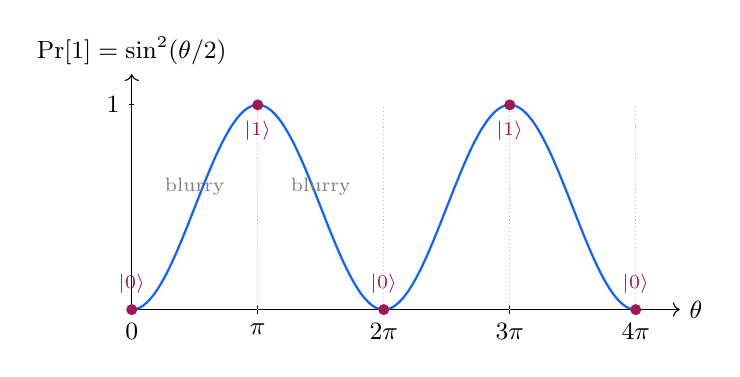
\begin{tikzpicture}[x=1.6cm,y=2.6cm]
  \draw[->] (0,0) -- (4.35,0) node[right,font=\small] {$\theta$};
  \draw[->] (0,0) -- (0,1.15) node[above,font=\small] {$\Pr[1]=\sin^2(\theta/2)$};
  \foreach \t/\l in {1/$\pi$,2/$2\pi$,3/$3\pi$,4/$4\pi$} {
    \draw (\t,0.02) -- (\t,-0.02) node[below,font=\small] {\l};
    \draw[gray!50,densely dotted] (\t,0) -- (\t,1);
  }
  \node[below,font=\small] at (0,-0.02) {$0$};
  \draw (0.02,1) -- (-0.02,1) node[left,font=\small] {$1$};
  \draw[keycol,thick] plot[domain=0:4,samples=240,variable=\t] ({\t},{sin(\t*90)*sin(\t*90)});
  \foreach \t in {0,2,4} { \fill[gatecol] (\t,0) circle (2pt); \node[above,font=\scriptsize,gatecol] at (\t,0.03) {$\ket{0}$}; }
  \foreach \t in {1,3}   { \fill[gatecol] (\t,1) circle (2pt); \node[below,font=\scriptsize,gatecol] at (\t,0.97) {$\ket{1}$}; }
  \node[font=\scriptsize,gray] at (0.5,0.6) {blurry};
  \node[font=\scriptsize,gray] at (1.5,0.6) {blurry};
\end{tikzpicture}
\caption{Probability of measuring $1$ after $\RX(\theta)\ket{0}$. The qubit is a definite basis
state only at whole multiples of $\pi$: $\ket{0}$ at even multiples, $\ket{1}$ at odd multiples.
Everywhere else it is a superposition (``blurry'').}
\label{fig:sin2}
\end{figure}

Three elementary properties of $\RX$ carry the whole derivation. Proofs are in
Appendix~\ref{app:proofs}.

\begin{lemma}[Clean angles]\label{lem:clean}
$\RX(\theta)\ket{0}$ is a computational basis state (up to a global phase) if and only if
$\theta$ is an integer multiple of $\pi$. Writing $\theta = m\pi$ with $m\in\Z$,
\[
\RX(m\pi)\ket{0} = \begin{cases}
 (-1)^{m/2}\,\ket{0} & m \text{ even},\\[2pt]
 -i\,(-1)^{(m-1)/2}\,\ket{1} & m \text{ odd}.
\end{cases}
\]
In words: the qubit ends in $\ket{b}$ where $b = m \bmod 2$ is the parity of $m$.
\end{lemma}

\begin{lemma}[Angles add]\label{lem:add}
$\RX(\theta_1)\,\RX(\theta_2) = \RX(\theta_1+\theta_2)$ for all real $\theta_1,\theta_2$.
Consequently all $\RX$ gates on the same wire commute, and a sequence of $\RX$ gates on one wire
is a single $\RX$ whose angle is the sum.
\end{lemma}

\begin{lemma}[Period $2\pi$ up to a sign]\label{lem:period}
$\RX(\theta + 2\pi) = -\RX(\theta)$, hence $\RX(\theta + 2\pi m) = (-1)^m\RX(\theta)$ for every
integer $m$.
\end{lemma}

\begin{keybox}[Crossing out $2\pi$]
Lemma~\ref{lem:period} says that a rotation by any multiple of $2\pi$ is the identity up to a
sign. When that sign is a global phase, it is invisible, and we may simply \emph{cross out} every
multiple of $2\pi$ from an angle. Section~\ref{sec:rigor} checks that in this circuit the sign is
indeed always global.
\end{keybox}

\subsection{The controlled rotation $\CRX$}

A controlled gate uses one qubit (the \emph{control}) to decide whether a gate acts on another
(the \emph{target}). The controlled-$\RX$ gate is defined on basis states by
\[
\CRX(\theta)\,\ket{c}\ket{t} =
\begin{cases}
\ket{0}\otimes\ket{t} & \text{if } c = 0 \ \text{(do nothing)},\\
\ket{1}\otimes\RX(\theta)\ket{t} & \text{if } c = 1 \ \text{(rotate the target)},
\end{cases}
\]
and extended linearly. Its $4\times4$ matrix is in Appendix~\ref{app:matrices}. The property we
need is almost tautological but is the crux of the construction:

\begin{keybox}[A controlled gate is a classical ``if'' when the control is definite]
If the control qubit is in a definite basis state $\ket{c}$ and the joint state is a product
state, then $\CRX(\theta)$ acts on the target exactly as $\RX(c\cdot\theta)$: it rotates by
$\theta$ when $c=1$ and by $0$ when $c=0$. The joint state remains a product state.
\end{keybox}

If instead the control is in a superposition, $\CRX$ rotates the target in one branch and not in
the other, and the two qubits become \emph{entangled}. Our derivation is arranged so that this
never happens for integer $\alpha$: every wire is finished, and therefore definite, before it is
used as a control.

% =====================================================================
\section{Turning the problem into arithmetic}\label{sec:arith}
% =====================================================================

We fix the eight knob values to be the integers $\alpha_n = n$, $n = 0,\dots,7$, and write $n$ in
binary as in \eqref{eq:binary}. The target for knob value $n$ is the state $\ket{b_0 b_1 b_2}$.

Suppose every gate in the circuit is an $\RX$ or $\CRX$ and, as promised, every control is
definite when it fires. Then by Lemma~\ref{lem:add} each wire $k$ receives one total rotation
angle $\Theta_k(n)$, and by Lemma~\ref{lem:clean} it ends in $\ket{b_k}$ precisely when
$\Theta_k(n)$ is a multiple of $\pi$ with parity $b_k$. Using the period from
Lemma~\ref{lem:period}, that condition is the congruence
\begin{equation}\label{eq:goal}
\boxed{\;\Theta_k(n) \eqmod{\pi\, b_k}\qquad\text{for } k = 0,1,2 \text{ and all } n = 0,\dots,7.\;}
\end{equation}

That is the whole problem: find gate angles, linear in the knob, whose total on each wire is
$\pi$ times that wire's own bit, modulo $2\pi$. The bits are not independent of the knob; they
are its binary digits. So multiply \eqref{eq:binary} by $\pi$:
\begin{equation}\label{eq:master}
\pi n = 4\pi b_0 + 2\pi b_1 + \pi b_2 .
\end{equation}
Everything below is a rearrangement of this one equation.

% =====================================================================
\section{The derivation, wire by wire}\label{sec:derivation}
% =====================================================================

\subsection{Wire 2: the least-significant bit}

We want $\Theta_2 \equiv \pi b_2 \pmod{2\pi}$. Look at \eqref{eq:master}: two of the three terms
on the right are multiples of $2\pi$, because $4\pi b_0 = 2\pi\cdot(2b_0)$ and
$2\pi b_1 = 2\pi\cdot b_1$ with $2b_0, b_1$ integers. Cross them out:
\[
\pi n = \cancel{4\pi b_0} + \cancel{2\pi b_1} + \pi b_2 \eqmod{\pi b_2}.
\]
So the angle $\pi n$ already satisfies the goal for wire 2. Since the knob is $\alpha = n$, this
is the angle $\pi\alpha$.

\begin{resultbox}
Apply a single free rotation $\RX(\pi\alpha)$ to wire 2. \hfill \code{qml.RX(np.pi * alpha, wires=2)}
\end{resultbox}

\noindent Intuitively, wire 2 flips once per unit of $\alpha$: $\ket{0},\ket{1},\ket{0},\ket{1},\dots$
It is the fastest wheel of an odometer.

\subsection{Wire 1: the middle bit}

We want $\Theta_1 \equiv \pi b_1$. Divide \eqref{eq:master} by $2$:
\[
\frac{\pi n}{2} = 2\pi b_0 + \pi b_1 + \frac{\pi b_2}{2}.
\]
Now only the first term is a multiple of $2\pi$. Cross it out:
\[
\frac{\pi n}{2} \eqmod{\pi b_1 + \frac{\pi}{2}\,b_2}.
\]
The angle $\pi n/2$ is therefore \emph{almost} right: it equals the target $\pi b_1$ plus an
unwanted $\frac{\pi}{2}b_2$. Solve for the target:
\begin{equation}\label{eq:wire1}
\pi b_1 \eqmod{\frac{\pi n}{2} \;-\; \frac{\pi}{2}\,b_2}.
\end{equation}
Read \eqref{eq:wire1} as an instruction. First rotate by $\pi n/2 = \pi\alpha/2$. Then subtract
$\pi/2$, but only when $b_2 = 1$. ``Rotate the target by $-\pi/2$ if and only if qubit 2 is
$\ket{1}$'' is exactly a $\CRX(-\pi/2)$ gate with control $q_2$ and target $q_1$. For this to work
as a classical ``if'', qubit 2 must already be in its final definite state, so the wire-2 gate
must come first.

\begin{resultbox}
Apply $\RX(\pi\alpha/2)$ to wire 1, then $\CRX(-\pi/2)$ with control wire 2 and target wire 1.\\[3pt]
\code{qml.RX(np.pi * alpha / 2, wires=1)}\\
\code{qml.CRX(-np.pi / 2, wires=[2, 1])}
\end{resultbox}

\noindent The odometer picture explains the correction. A half-speed wheel that turns
continuously does not \emph{click}: when the fast wheel shows $1$, the slow wheel has drifted half
a notch and is blurry. The controlled gate removes exactly that half notch.

\subsection{Wire 0: the most-significant bit}

We want $\Theta_0 \equiv \pi b_0$. Divide \eqref{eq:master} by $4$:
\[
\frac{\pi n}{4} = \pi b_0 + \frac{\pi b_1}{2} + \frac{\pi b_2}{4}.
\]
This time nothing is a multiple of $2\pi$, so nothing can be crossed out. Solve for the target:
\begin{equation}\label{eq:wire0}
\pi b_0 = \frac{\pi n}{4} \;-\; \frac{\pi}{2}\,b_1 \;-\; \frac{\pi}{4}\,b_2 .
\end{equation}
Again read it as an instruction: rotate by $\pi\alpha/4$; subtract $\pi/2$ if qubit 1 is
$\ket{1}$; subtract $\pi/4$ if qubit 2 is $\ket{1}$. Two controlled gates, both targeting wire 0.
Both controls must be definite, so these gates come after wires 1 and 2 are finished. The two
corrections are $\RX$ gates on the same wire, so by Lemma~\ref{lem:add} their order does not
matter.

\begin{resultbox}
Apply $\RX(\pi\alpha/4)$ to wire 0, then $\CRX(-\pi/4)$ controlled by wire 2 and $\CRX(-\pi/2)$
controlled by wire 1, both targeting wire 0.\\[3pt]
\code{qml.RX(np.pi * alpha / 4, wires=0)}\\
\code{qml.CRX(-np.pi / 4, wires=[2, 0])}\\
\code{qml.CRX(-np.pi / 2, wires=[1, 0])}
\end{resultbox}

\subsection{The architecture is forced}

Collecting the three results gives exactly Figure~\ref{fig:circuit}. Nothing was chosen freely:
\begin{itemize}[nosep]
\item the free rotation on wire $k$ has angle $\pi\alpha/2^{\,2-k}$, because isolating bit $b_k$
      means dividing the binary expansion by $2^{\,2-k}$;
\item the correction from a lower wire $j>k$ onto wire $k$ has angle $-\pi/2^{\,j-k}$, because
      that is the coefficient of $b_j$ after the division;
\item the gate order is dictated by the requirement that every control be definite when it fires.
\end{itemize}

\begin{remark}
The pattern ``divide by powers of two, then undo the lower bits with controlled rotations of
$\pi/2^{\,j-k}$'' is the same bookkeeping that appears in the quantum Fourier transform, where
controlled phase rotations by $\pi/2^{\,j-k}$ implement a binary expansion. Here the rotations
are about the $x$ axis and act on populations rather than phases, but the arithmetic is identical.
\end{remark}

\begin{remark}[Why the factor $\pi$ sits inside the gates]
One could equally use $\RX(\alpha)$, $\RX(\alpha/2)$, $\RX(\alpha/4)$ with knob values
$\alpha_n = n\pi$. But $7\pi \approx 21.99$ lies outside the required interval $[0,10]$. Putting
$\pi$ inside the gate rescales the knob so that the eight values are $0,1,\dots,7$.
\end{remark}

% =====================================================================
\section{Checking all eight inputs}\label{sec:check}
% =====================================================================

Table~\ref{tab:check} lists, for every $n$, the total angle on each wire in units of $\pi$. The
``free'' column is the uncontrolled rotation, the ``corr.'' column is the sum of the controlled
corrections that fire, and the ``net'' column is their sum. Comparing the parity of each net
multiple of $\pi$ with the corresponding bit confirms \eqref{eq:goal}. In closed form,
\[
\Theta_2 = \pi n, \qquad
\Theta_1 = \frac{\pi n}{2} - \frac{\pi}{2}b_2 = \pi(b_1 + 2b_0), \qquad
\Theta_0 = \frac{\pi n}{4} - \frac{\pi}{2}b_1 - \frac{\pi}{4}b_2 = \pi b_0 .
\]

\begin{table}[ht]
\centering\small
\setlength{\tabcolsep}{5pt}
\begin{tabular}{c c c | c c c | c c c | c}
\toprule
$n$ & $b_0b_1b_2$ & $\Theta_2/\pi$ & \multicolumn{3}{c|}{wire 1: $\Theta_1/\pi$} & \multicolumn{3}{c|}{wire 0: $\Theta_0/\pi$} & output \\
    &             & $=n$           & free $n/2$ & corr. $-b_2/2$ & net & free $n/4$ & corr. $-b_1/2-b_2/4$ & net & $\ket{b_0b_1b_2}$\\
\midrule
0 & 000 & 0 & 0    & 0      & 0 & 0    & 0      & 0 & $\ket{000}$\\
1 & 001 & 1 & 1/2  & $-1/2$ & 0 & 1/4  & $-1/4$ & 0 & $\ket{001}$\\
2 & 010 & 2 & 1    & 0      & 1 & 1/2  & $-1/2$ & 0 & $\ket{010}$\\
3 & 011 & 3 & 3/2  & $-1/2$ & 1 & 3/4  & $-3/4$ & 0 & $\ket{011}$\\
4 & 100 & 4 & 2    & 0      & 2 & 1    & 0      & 1 & $\ket{100}$\\
5 & 101 & 5 & 5/2  & $-1/2$ & 2 & 5/4  & $-1/4$ & 1 & $\ket{101}$\\
6 & 110 & 6 & 3    & 0      & 3 & 3/2  & $-1/2$ & 1 & $\ket{110}$\\
7 & 111 & 7 & 7/2  & $-1/2$ & 3 & 7/4  & $-3/4$ & 1 & $\ket{111}$\\
\bottomrule
\end{tabular}
\caption{Total rotation angle on each wire, in units of $\pi$, for the eight knob values. Every
net entry is an integer, and its parity equals the corresponding bit: wire 2 is odd exactly for
odd $n$, wire 1 is odd exactly for $n\in\{2,3,6,7\}$, wire 0 is odd exactly for $n\ge4$. Without
the corrections, the free columns contain half- and quarter-integers, i.e.\ superpositions.}
\label{tab:check}
\end{table}

Notice the entries $\Theta_1/\pi = 2$ and $3$ for $n\ge4$: these are the cases where a $2\pi$ was
crossed out. Lemma~\ref{lem:period} says the state picks up a factor $-1$ there, which is a global
phase because the register is a product state.

% =====================================================================
\section{One input followed state by state: $n = 3$}\label{sec:example}
% =====================================================================

Take $\alpha = 3$, so the target is $\ket{011}$ and the gate angles are $3\pi$, $3\pi/2$,
$-\pi/2$, $3\pi/4$, $-\pi/4$, $-\pi/2$. We write the state after each gate, keeping every phase.
Recall $\cos\frac{3\pi}{4} = -\frac{\sqrt2}{2}$, $\sin\frac{3\pi}{4} = \frac{\sqrt2}{2}$,
$\cos\frac{3\pi}{8}\approx 0.3827$, $\sin\frac{3\pi}{8}\approx 0.9239$.

\begin{enumerate}[label=\textbf{Gate \arabic*.},leftmargin=2.1cm,itemsep=5pt]
\item[\textbf{Start.}] $\ket{\psi_0} = \ket{000}$.
\item $\RX(3\pi)$ on $q_2$. By \eqref{eq:rx0}, $\RX(3\pi)\ket{0} = \cos\frac{3\pi}{2}\ket{0} - i\sin\frac{3\pi}{2}\ket{1} = 0\cdot\ket{0} - i(-1)\ket{1} = i\ket{1}$.
      \[\ket{\psi_1} = i\,\ket{001}.\]
      Qubit 2 is definitely $1$ (the factor $i$ is a global phase). This is the first $2\pi$
      cross-out in action: $\RX(3\pi) = -\RX(\pi)$, and $\RX(\pi)\ket{0} = -i\ket{1}$.
\item $\RX(3\pi/2)$ on $q_1$. $\RX(\tfrac{3\pi}{2})\ket{0} = -\frac{\sqrt2}{2}\ket{0} - i\frac{\sqrt2}{2}\ket{1}$.
      \[\ket{\psi_2} = i\Big(-\tfrac{\sqrt2}{2}\ket{001} - i\tfrac{\sqrt2}{2}\ket{011}\Big)
                     = -\tfrac{i}{\sqrt2}\ket{001} + \tfrac{1}{\sqrt2}\ket{011}.\]
      Qubit 1 is now blurry: probabilities $\frac12$ and $\frac12$. This is the ``half notch''
      caused by $b_2 = 1$.
\item $\CRX(-\pi/2)$, control $q_2$, target $q_1$. Qubit 2 is $1$ in every term, so the gate
      applies $\RX(-\pi/2)$ to qubit 1 in every term. By Lemma~\ref{lem:add} the total on qubit 1
      is $\RX(\tfrac{3\pi}{2} - \tfrac{\pi}{2}) = \RX(\pi)$, and $\RX(\pi)\ket{0} = -i\ket{1}$.
      \[\ket{\psi_3} = i\cdot(-i)\,\ket{011} = \ket{011}.\]
      Both lower wires are finished and definite. One can also verify the step directly on the
      qubit-1 vector:
      \[\RX(-\tfrac{\pi}{2})\begin{pmatrix}-\tfrac{\sqrt2}{2}\\ -i\tfrac{\sqrt2}{2}\end{pmatrix}
        = \tfrac{\sqrt2}{2}\begin{pmatrix}1 & i\\ i & 1\end{pmatrix}\begin{pmatrix}-\tfrac{\sqrt2}{2}\\ -i\tfrac{\sqrt2}{2}\end{pmatrix}
        = \begin{pmatrix}0\\ -i\end{pmatrix}.\]
\item $\RX(3\pi/4)$ on $q_0$.
      \[\ket{\psi_4} = \cos\tfrac{3\pi}{8}\ket{011} - i\sin\tfrac{3\pi}{8}\ket{111}
                     \approx 0.3827\ket{011} - 0.9239\,i\ket{111}.\]
      Probabilities $0.146$ and $0.854$. Qubit 0 carries the unwanted
      $\frac{\pi}{2}b_1 + \frac{\pi}{4}b_2 = \frac{3\pi}{4}$ on top of its target $0$.
\item $\CRX(-\pi/4)$, control $q_2 = 1$, target $q_0$. Total on qubit 0: $\RX(\tfrac{3\pi}{4} - \tfrac{\pi}{4}) = \RX(\tfrac{\pi}{2})$.
      \[\ket{\psi_5} = \tfrac{1}{\sqrt2}\ket{011} - \tfrac{i}{\sqrt2}\ket{111}.\]
\item $\CRX(-\pi/2)$, control $q_1 = 1$, target $q_0$. Total on qubit 0: $\RX(\tfrac{\pi}{2} - \tfrac{\pi}{2}) = \RX(0) = I$.
      \[\ket{\psi_6} = \ket{011}.\]
\end{enumerate}
The final state is exactly the target, here even with phase $+1$. Measuring returns $011$ with
probability one, and the probability vector has a $1$ in position $3$.

% =====================================================================
\section{Making ``cross out $2\pi$'' rigorous}\label{sec:rigor}
% =====================================================================

The informal rule ``a $2\pi$ rotation does nothing'' is not literally true for a qubit:
$\RX(2\pi) = -I$ (Lemma~\ref{lem:period}). A sign is harmless only when it multiplies the entire
state. Here is why that is always the case in this circuit for integer $\alpha$.

\begin{theorem}\label{thm:product}
For every integer $n$, the state of the register after each of the six gates is a product state
of the form $e^{i\varphi}\ket{s_0}\otimes\ket{s_1}\otimes\ket{s_2}$, with each $\ket{s_k}$ a
single-qubit state and $e^{i\varphi}$ a global phase. Consequently every sign produced by
Lemma~\ref{lem:period} is global, and the measurement probabilities after the sixth gate are those
of $\ket{b_0b_1b_2}$.
\end{theorem}

\begin{proof}
Induction over the gates. The initial state $\ket{000}$ is a product state. An $\RX$ gate acts on
one factor and preserves the product form. For a $\CRX$ gate we check that its control is a
definite basis state at that moment, so that the gate acts as $\RX(c\theta)$ on the target factor
(the boxed property in Section~\ref{sec:qm}) and again preserves the product form:
\begin{itemize}[nosep]
\item Gate 3 is controlled by $q_2$ after gate 1, whose total angle $\pi n$ is a multiple of
      $\pi$, so $q_2 = \ket{b_2}$ up to phase by Lemma~\ref{lem:clean}.
\item Gates 5 and 6 are controlled by $q_2$ and by $q_1$ after gate 3. The total on $q_1$ is
      $\pi n/2 - \pi b_2/2 = \pi(b_1+2b_0)$, a multiple of $\pi$, so $q_1 = \ket{b_1}$ up to
      phase.
\end{itemize}
Finally the total on $q_0$ is $\pi n/4 - \pi b_1/2 - \pi b_2/4 = \pi b_0$. Each factor is a basis
state up to a phase, and a product of phases is a single global phase.
\end{proof}

\begin{remark}
For non-integer $\alpha$ the controls are superpositions when they fire, the register becomes
entangled, and the relative signs from $\RX(2\pi)=-I$ do matter. The challenge never evaluates
those states for correctness; it only requires the map $\alpha\mapsto$ probabilities to be
continuous, which holds because every matrix entry is a continuous function of $\alpha$.
\end{remark}

% =====================================================================
\section{Why controlled gates cannot be avoided}\label{sec:impossible}
% =====================================================================

It is natural to ask whether a cleverer choice of three \emph{uncontrolled} rotations,
$\RX(c_0\alpha)$, $\RX(c_1\alpha)$, $\RX(c_2\alpha)$ with real constants $c_k$, could reach all
eight states for some eight knob values. It cannot.

\begin{theorem}\label{thm:impossible}
There are no real constants $c_0,c_1,c_2$ and real numbers $\alpha_0,\dots,\alpha_7$ such that
the product circuit $\RX(c_0\alpha)\otimes\RX(c_1\alpha)\otimes\RX(c_2\alpha)$ applied to
$\ket{000}$ yields $\ket{b_0b_1b_2}$ (up to phase) at $\alpha = \alpha_n$ for every $n$.
\end{theorem}

\begin{proof}
Suppose such constants and values exist. By Lemma~\ref{lem:clean}, reaching a basis state at
$\alpha$ requires $c_k\alpha = \pi m_k$ with $m_k\in\Z$ and $m_k \equiv b_k \pmod 2$ for each $k$.

Reaching $\ket{100}$ requires $c_0 \neq 0$ (otherwise wire 0 never leaves $\ket{0}$), and
reaching $\ket{001}$ requires $c_2\neq0$. Let $a$ be the knob value for $\ket{001}$ and $a'$ the
one for $\ket{100}$. Neither is zero, since $\alpha = 0$ gives $\ket{000}$.

At $\alpha = a$: $c_0 a = \pi e$ with $e$ even and $c_2 a = \pi o$ with $o$ odd. Dividing,
$c_0/c_2 = e/o$.

At $\alpha = a'$: $c_0 a' = \pi o'$ with $o'$ odd and $c_2 a' = \pi e'$ with $e'$ even, and
$e'\neq0$ because $c_2\neq0$ and $a'\neq0$. Dividing, $c_0/c_2 = o'/e'$.

Hence $e/o = o'/e'$, so $e\,e' = o\,o'$. The left side is even and the right side is odd, a
contradiction.
\end{proof}

The theorem says more than ``the naive attempt fails'': any single layer of $x$-rotations with
angles proportional to one knob is blocked by parity. Some gate must let a wire \emph{read} the
other wires, and the controlled corrections derived in Section~\ref{sec:derivation} are the
minimal way to do so. (The same proof works for $\RX$ replaced by $\RY$, or any fixed rotation
axis in the equatorial plane, since Lemma~\ref{lem:clean} holds for those as well.)

% =====================================================================
\section{Summary}
% =====================================================================

\begin{enumerate}[nosep]
\item A rotation $\RX(\theta)$ from $\ket{0}$ is a basis state iff $\theta\in\pi\Z$, and it is
      $\ket{1}$ iff $\theta/\pi$ is odd. Angles on one wire add. A multiple of $2\pi$ is a global
      sign.
\item The task is therefore: make each wire's total angle congruent to $\pi\times$(its own bit)
      modulo $2\pi$, for knob values $n = 0,\dots,7$.
\item Multiply the binary expansion $n = 4b_0+2b_1+b_2$ by $\pi$ and divide by $1$, $2$, $4$.
      Cross out multiples of $2\pi$ and move the remaining lower-bit terms to the other side:
      \[
      \pi b_2 \equiv \pi\alpha,\qquad
      \pi b_1 \equiv \tfrac{\pi\alpha}{2} - \tfrac{\pi}{2}b_2,\qquad
      \pi b_0 = \tfrac{\pi\alpha}{4} - \tfrac{\pi}{2}b_1 - \tfrac{\pi}{4}b_2 .
      \]
\item Each term $\pi\alpha/2^{j}$ is a free rotation; each term $-\frac{\pi}{2^{j}}b_k$ is a
      controlled rotation with control $q_k$. Controls must be definite when they fire, which
      fixes the gate order. The result is Figure~\ref{fig:circuit} with coefficients $0,\dots,7$.
\item Uncontrolled rotations alone can never work, by a parity argument.
\end{enumerate}

\appendix
% =====================================================================
\section{Matrices}\label{app:matrices}
% =====================================================================

With $c = \cos\frac{\theta}{2}$ and $s = \sin\frac{\theta}{2}$,
\[
\RX(\theta) = \begin{pmatrix} c & -is\\ -is & c\end{pmatrix},\qquad
\CRX(\theta) = \begin{pmatrix} 1&0&0&0\\ 0&1&0&0\\ 0&0&c&-is\\ 0&0&-is&c\end{pmatrix}
             = \ket{0}\!\bra{0}\otimes I + \ket{1}\!\bra{1}\otimes \RX(\theta),
\]
where in $\CRX$ the control is the first (left) tensor factor and the target the second. For a
gate acting on wire $k$ of a three-qubit register, the full $8\times8$ matrix is the Kronecker
product with identities in the other slots, e.g.\ $\RX$ on wire 1 is $I\otimes\RX(\theta)\otimes I$,
and $\CRX$ with control $2$ and target $0$ is
$I\otimes I\otimes\ket{0}\!\bra{0} \;+\; \RX(\theta)\otimes I\otimes\ket{1}\!\bra{1}$.
This is exactly how the interactive simulator in the repository builds its operators.

% =====================================================================
\section{Proofs of the three lemmas}\label{app:proofs}
% =====================================================================

\begin{proof}[Proof of Lemma~\ref{lem:clean}]
From \eqref{eq:rx0}, $\RX(\theta)\ket{0}$ has probabilities $\cos^2\frac{\theta}{2}$ and
$\sin^2\frac{\theta}{2}$. It is a basis state iff one of them is $0$, i.e.\ iff
$\sin\frac{\theta}{2} = 0$ or $\cos\frac{\theta}{2} = 0$, i.e.\ iff $\frac{\theta}{2}\in\frac{\pi}{2}\Z$,
i.e.\ iff $\theta\in\pi\Z$. For $\theta = m\pi$: if $m$ is even, $\sin\frac{m\pi}{2}=0$ and
$\cos\frac{m\pi}{2} = (-1)^{m/2}$; if $m$ is odd, $\cos\frac{m\pi}{2}=0$ and
$\sin\frac{m\pi}{2} = (-1)^{(m-1)/2}$. Inserting into \eqref{eq:rx0} gives the stated formulas.
\end{proof}

\begin{proof}[Proof of Lemma~\ref{lem:add}]
Write $\RX(\theta) = \cos\frac{\theta}{2}\,I - i\sin\frac{\theta}{2}\,X$ with
$X = \begin{pmatrix}0&1\\1&0\end{pmatrix}$, $X^2 = I$. Then
\begin{align*}
\RX(\theta_1)\RX(\theta_2)
&= \big(\cos\tfrac{\theta_1}{2}\cos\tfrac{\theta_2}{2} - \sin\tfrac{\theta_1}{2}\sin\tfrac{\theta_2}{2}\big) I
 - i\big(\sin\tfrac{\theta_1}{2}\cos\tfrac{\theta_2}{2} + \cos\tfrac{\theta_1}{2}\sin\tfrac{\theta_2}{2}\big) X\\
&= \cos\tfrac{\theta_1+\theta_2}{2}\, I - i \sin\tfrac{\theta_1+\theta_2}{2}\, X = \RX(\theta_1+\theta_2),
\end{align*}
by the angle-addition formulas. Commutativity follows because addition of angles commutes.
\end{proof}

\begin{proof}[Proof of Lemma~\ref{lem:period}]
$\cos\frac{\theta+2\pi}{2} = \cos(\frac{\theta}{2}+\pi) = -\cos\frac{\theta}{2}$ and likewise
$\sin(\frac{\theta}{2}+\pi) = -\sin\frac{\theta}{2}$. Both entries of \eqref{eq:rx} change sign,
so $\RX(\theta+2\pi) = -\RX(\theta)$. Iterating $m$ times gives $(-1)^m$.
\end{proof}

% =====================================================================
\section{The circuit in OpenQASM 3.0}
% =====================================================================

In OpenQASM the parameter is the angle itself, so the eight basis states sit at
$\alpha = 0,\pi,2\pi,\dots,7\pi$; the PennyLane coefficient is the multiple $n$.
\begin{quote}\small
\begin{verbatim}
OPENQASM 3.0;
include "stdgates.inc";
angle alpha = pi;
qubit q[3];
bit c[3];

rx(alpha) q[2];              // wire 2 (LSB)
rx(alpha / 2) q[1];          // wire 1
crx(-pi / 2) q[2], q[1];
rx(alpha / 4) q[0];          // wire 0 (MSB)
crx(-pi / 4) q[2], q[0];
crx(-pi / 2) q[1], q[0];

c = measure q;
\end{verbatim}
\end{quote}

\end{document}
